\documentclass{article}
\usepackage[utf8]{inputenc} % allow utf-8 input
\usepackage[main=english,russian]{babel}	
\usepackage{arxiv}

\usepackage[T1]{fontenc}    % use 8-bit T1 fonts
\usepackage{hyperref}       % hyperlinks
\usepackage{url}            % simple URL typesetting
\usepackage{booktabs}       % professional-quality tables
\usepackage{amsfonts}       % blackboard math symbols
\usepackage{nicefrac}       % compact symbols for 1/2, etc.
\usepackage{microtype}      % microtypography
\usepackage{lipsum}         % Can be removed after putting your text content
\usepackage{graphicx}
\usepackage{natbib}
\usepackage{doi}
\usepackage{amsmath}
\usepackage{algorithm}
\usepackage{algpseudocode}
\usepackage{amsthm}
\usepackage{amssymb}
\newtheorem{theorem}{Theorem}

\title{On the problem of repeated supervised learning}

%\date{September 9, 1985}	% Here you can change the date presented in the paper title
%\date{} 					% Or removing it

\author{
    Andrey S. Veprikov\\
	Department of Intelligent Systems\\
	MIPT\\
	Dolgoprudny, Russia \\
	\texttt{veprikov.as@phystech.edu} 
    \And
    Anton S. Kritanlov\\
    HSE University\\
    Moscow, Russia\\
    \texttt{akhritankov@hse.ru}\\
    \And
    Alexander P. Afanasyev \\
    IITP\\
    Moscow, Russia}

\date{}

% Uncomment to override  the `A preprint' in the header
%\renewcommand{\headeright}{Technical Report}
%\renewcommand{\undertitle}{Technical Report}
\renewcommand{\shorttitle}{On the problem of repeated supervised learning}

%%% Add PDF metadata to help others organize their library
%%% Once the PDF is generated, you can check the metadata with
%%% $ pdfinfo template.pdf

\begin{document}
\maketitle

\begin{abstract}

    In this research paper, we delve into the intricacies of continuous learning artificial intelligence systems as they interact with and influence their environment. We develop a mathematical model to examine the process of repeated and multiple learning, prediction, and dataset updating. Our investigation of this process is based on the principles of functional analysis and probability theory, which is a novel approach to this problem. We aim to conduct several synthetic experiments based on our findings, hoping to contribute to a better understanding of the behavior of continuous learning AI systems.

\end{abstract}


% keywords can be removed
\keywords{Machine learning \and Continuous machine learning \and Repeated learning}

\section{Introduction} \label{Introduction}

    In this paper we consider the problem of repeated supervised learning \begin{otherlanguage}{russian}(многократное машинное обучение)\end{otherlanguage}, in which the training sample is not fixed, but is updated depending on the predictions of the trained model on the test sample \cite{ma2020machine, khritankov2021existence, jiang2019degenerate}. In many applications, the use of multiple learning techniques can actually lead to suboptimal results. Our main goal was to present a mathematical theory that explains why combining multiple learning algorithms can sometimes hinder their effectiveness. Repeated supervised learning appears in many machine learning applications, for example in recommendation systems \cite{khritankov2021existence, sinha2016deconvolving}, healthcare \cite{adam2020hidden} and predictive policing \cite{ensign2018runaway}. 

    The object of our research will be the set $\mathbf{R}$ of distribution density functions

    \begin{equation}
        \label{R}
        \mathbf{R} := \left\{f : \mathbb{R}^n \rightarrow \mathbb{R}_+ ~\text{and}~ \int\limits_{\mathbb{R}^n}f(x)dx = 1\right\},
    \end{equation}

    and a mapping $\text{D}$, a feedback loop mapping, that includes training a model, forming predictions on a test sample and mixing predictions into a training sample, as a result of which the distribution of features changes.

    A range of problems, that we are considering in this paper are conditions under which $\text{D}$ translates $\mathbf{R}$ into $\mathbf{R}$, conditions when $\text{D}$ is a contraction mapping and its fixed point existence conditions.

    Main contributions ...
    
    Structure of this paper are as follows. In Section \ref{Related_work} we compare our article with the works of other authors and show its novelty to the literature. In Section \ref{Problem_statement} we build a mathematical model for the process of multiple learning, prediction and updating of the sample and outline the main questions, the answers to which we explore in Section \ref{Main_results}. In Section \ref{Main_results} we provide our main contributions for the mapping $\text{D}$. In Section \ref{Experiments}, based on the results from Section \ref{Main_results}, we conduct some synthetic experiments.

\section{Related work} \label{Related_work}    

    The problem we study is somewhat related to the feedback loops \cite{khritankov2021hidden, khritankov2021existence} -- an observable change in the distribution of input data that occurs over time, because of user interaction with the system. According to Conjecture 1 from \cite{khritankov2021hidden} the positive feedback loop in a system $\text{D} : R \rightarrow R$ exists if $\text{D}$ is a contraction mapping, but this conjecture was not proved.

    Also our problem is connected with dynamical systems, which are studied in \cite{katok1995introduction, nemytskii2015qualitative}, but all these works consider continuous time, and in our work it should be discrete.

    Some authors analyzed Markov processes from the point of view of dynamical systems \cite{tarlowski2017global, vershik2005does}. But in Markov chain the future of the process does not depend on the past. Other authors \cite{varvenne2019rate, pap1996fixed} studied stochastic dynamics systems in general.

    An important contribution of this paper is that ...

\section{Problem statement} \label{Problem_statement}

    We consider $\mathbf{R}$ \eqref{R} -- the set of distribution density functions and a mapping $\text{D}$ representing an algorithm for training a model, forming predictions on a test sample and mixing predictions into a training sample, as a result of which the distribution of features changes.

    Let's consider an autonomous (time-independent explicitly) discrete dynamical system. There is a dedicated variable - the step number, which increases, at step $t$ and $t+1$ of which the ratio is fulfilled

    \begin{equation*}
        f_{t+1}(x) = \text{D}(f_t)(x), \quad \text{for}~ \forall x \in \mathbb{R}^n,
    \end{equation*}

    where $\text{D}$ becomes an evolution operator on the space of the specified functions $f$ and the initial function $f_0(x)$ is known. Generally speaking, $\text{D}$ can be an arbitrary mapping, not necessarily smooth or continuous.

    In this paper we consider the following research questions:

    \begin{enumerate}
        \item[\textbf{1.}]  What are the conditions so that the mapping $\text{D}$ becomes a transformation $\mathbf{R}$ into $\mathbf{R}$? 

        \item[\textbf{2.}] Under what conditions the mapping $\text{D}$ is a contraction mapping?

        \item[\textbf{3.}] Under what conditions the mapping $\text{D}$ has a fixed point?
    \end{enumerate}

    Let's analyze the importance of each question. We consider $\text{D}$ as operator of changing distribution of our dataset, so it has to transform $\mathbf{R}$ into $\mathbf{R}$. If $\text{D}$ is a contraction mapping, then for any starting function $f_0$ after a sufficiently large T, the result of our algorithm after $T$ steps would be $D^T(f_0) = f^*$, where $f^*$ is a fixed point, so after $T$ steps metrics of our algorithm cannot be improved. If $\text{D}$ has a fixed point $f$, when if $f_0 = f$ and we cannot improve our metrics as well.


\section{Main results} \label{Main_results}

    In this section we will provide several theorems on operator $\text{D}$ to answer questions 1-3.

    \textbf{Notation:} In this paper we will use the common notations: the $L_1(\mathbb{R}^n)$-norm of function $f$:

    \begin{equation*}
        \|f\|_1 := \int\limits_{\mathbb{R}^n} |f(x)| dx \quad \text{ and } \quad L_1(\mathbb{R}^n) := \left\{f : \mathbb{R}^n \to \mathbb{R} ~|~ \|f\|_1 < + \infty\right\}
    \end{equation*}

    The $L_{\infty}(\mathbb{R}^n)$-norm of function $f$:

    \begin{equation*}
        \|f\|_{\infty} := \underset{x \in \mathbb{R}^n}{\text{esssup}}\{f(x)\} := \inf\{C \geq 0 ~|~ |f(x)| \leq C \text{ for almost every } x \in \mathbb{R}^n\} \quad \text{ and } \quad L_{\infty}(\mathbb{R}^n) := \left\{f : \mathbb{R}^n \to \mathbb{R} ~|~ \|f\|_{\infty} < + \infty\right\}
    \end{equation*}

    \begin{theorem}[Fact] \label{Th1}
        If $f: \mathbb{R}^n \to \mathbb{R}$ such that $f(x) \geq 0$ for almost every $x \in \mathbb{R}^n$ and $\|f\|_1 = \int\limits_{\mathbb{R}^n} f(x) dx = 1$, then there exists a random vector $\mathbf{\xi}$, for which $f$ will be a density distribution function.
    \end{theorem}

    Exactly on the basis of Theorem \ref{Th1} we define $\mathbf{R}$ \eqref{R} in this way.

    \begin{theorem}[Assumptions for $\text{D}: \mathbf{R} \to \mathbf{R}$] \label{Th2}
        If $\|\text{D}\|_1 = 1, \forall f \in \mathbf{R} \hookrightarrow \text{D}(f)(x) \geq 0$ for almost every $x \in \mathbb{R}^n$, and exists $\text{D}^{-1}$ such that $\|\text{D}^{-1}\|_1 \leq 1$, then $\text{D} : \mathbf{R} \to \mathbf{R}$.
    \end{theorem}
    \begin{proof}
        To begin with, let us note that if $\text{D}: \mathbf{R} \to \mathbf{R}$, then $\|\text{D}\|_1 = 1$, because by definition of operator norm:

        \begin{equation*}
            \|\text{D}\|_1 \overset{def}{=} \underset{\|f\|_1 = 1}{\sup}\left\{\|\text{D}(f)\|_1\right\}
        \end{equation*}

        And if $f$ such that $\|f\|_1 = 1$ then $|f| \in \mathbf{R}$ and, because $\text{D}: \mathbf{R} \to \mathbf{R}$, $\|\text{D}(|f|)\|_1 = 1$. But $\|\text{D}\|_1 = 1$ is only a necessary but not a sufficient condition.

        If $\|\text{D}\|_1 = 1$, then $\forall f \in \mathbf{R} \hookrightarrow \text{D}(f) \leq 1$. If $\exists f_0 \in \mathbf{R}$ such that $\|\text{D}(f_0)\|_1 < 1$, then we get a contradiction because

        \begin{equation*}
            \|D^{-1}\|_1 \overset{def}{=} \underset{\|f\|_1 \neq 0}{\sup}\left\{\dfrac{\|\text{D}^{-1}(f)\|_1}{\|f\|_1}\right\} 
            \geq \left[f_1 = \text{D}(f_0)\right] \geq
            \dfrac{\|\text{D}^{-1}(f_1)\|_1}{\|f_1\|_1} = 
            \dfrac{\|\text{D}^{-1}(\text{D}(f_0))\|_1}{\|\text{D}(f_0)\|_1} = 
            \dfrac{\|f_0\|_1}{\|\text{D}(f_0)\|_1} = \dfrac{1}{\|\text{D}(f_0)\|_1} > 1
        \end{equation*}

        But we assume that $\|\text{D}^{-1}\|_1 \leq 1$. So $\forall f \in \mathbf{R} \hookrightarrow \|\text{D}(f)\|_1 = 1$.

        But according to Theorem \ref{Th1} to $\text{D} : \mathbf{R} \to \mathbf{R}$ we also need second assumption: $\forall f \in \mathbf{R} \hookrightarrow \text{D}(f)(x) \geq 0$ for almost every $x \in \mathbb{R}^n$.
        
    \end{proof}

    In our experiment it often difficult to calculate $\text{D}^{-1}$ and especially it's norm, so we make a different assumptions. We assume that our data sample describes the distribution function sufficiently well, so approximating the density function by our sample closely enough approaches the true density function of the data distribution. And if we consider $\text{D}$ as algorithm for training a model, forming predictions on a test sample and mixing predictions into a training sample, then $\text{D} : \mathbf{R} \to \mathbf{R}$ by constructing our density functions of data distributions.

    % Theorem 3 is wrong 
    \if 0
    \begin{theorem}[Inequality on $\|\text{D}\|_{\infty}$] \label{Th3}
        If $\text{D} : \mathbf{R} \cap L_{\infty}(\mathbb{R}^n) \to \mathbf{R} \cap L_{\infty}(\mathbb{R}^n)$ and , then $\|\text{D}\|_{\infty} \geq 1$
    \end{theorem}

    \begin{proof}
        Let us first write out two Herder's inequality: $\forall f \in \mathbf{R} \cap L_{\infty}(\mathbb{R}^n)$ it is fulfilled that

        \begin{equation*}
            \|f\|_1 \cdot \|\text{D}(f)\|_{\infty} \geq \|f \cdot \text{D}(f)\|_1
        \end{equation*}
        \begin{equation*}
            \|f\|_{\infty} \cdot \|\text{D}(f)\|_1 \geq \|f \cdot \text{D}(f)\|_1
        \end{equation*}

        Note that $\|f\|_1 = \|\text{D}(f)\|_1 = 1$ and $f, \text{D}(f) \in \mathbf{R} \cap L_{\infty}(\mathbb{R}^n)$ because $\text{D} : \mathbf{R} \cap L_{\infty}(\mathbb{R}^n) \to \mathbf{R} \cap L_{\infty}(\mathbb{R}^n)$. Let's add these two inequalities together and get

        \begin{equation*}
            \|\text{D}(f)\|_{\infty} + \|f\|_{\infty} \geq 2 \|f \cdot \text{D}(f)\|_1
        \end{equation*}

        Using common inequality on operators norm $\|\text{D}(f)\| \leq \|\text{D}\| \cdot \|f\| ~\forall f \in \mathbf{R}$ we get

        \begin{equation} \label{tmp1}
            (1 + \|\text{D}\|_{\infty}) \|f\|_{\infty} \geq 2 \|f \cdot \text{D}(f)\|_1
        \end{equation}

        Inequality \eqref{tmp1} is fulfilled for any $f \in \mathbf{R} \cap L_{\infty}(\mathbb{R}^n)$. Let's consider for any $\delta > 0$

        \begin{equation*}
            f_{\delta}(x) := V_n(\delta) \cdot \textbf{1}_{B(1/\delta)}(x),
        \end{equation*}

        where $B(1/\delta) := \mathbb{B}^n_{\|\cdot\|_2}(1/\delta) = \{x \in \mathbb{R}^n ~|~ \|x\|_2 \leq 1/\delta$\} -- the euclidean ball with radius $1/\delta$, $\textbf{1}_{A}(x)$ -- characteristic function of a set $A$ and $V_n(\delta) = \frac{\pi^{n/2}}{\Gamma(n/2+1)} \cdot \delta^n$ -- the volume of $\mathbb{B}^n_{\|\cdot\|_2}(\delta)$. In the formula for the volume of an $n$-dimensional Euclidean ball we are interested only in the fact that $V_n(\delta) = \kappa(n) \cdot \delta^n$, so we can calculate

        \begin{equation*}
            \|f_{\delta}\|_1 = \int\limits_{\mathbb{R}^n} |f_{\delta}(x)|dx = V_n(\delta) \cdot \int\limits_{B(1/\delta)}dx = V_n(\delta) \cdot V_n(1/\delta) = 1
            \quad \text{ and } \quad \|f_{\delta}\|_{\infty} = V_n(\delta)
        \end{equation*}

        So, $\forall \delta > 0 \hookrightarrow f_{\delta} \in \mathbf{R} \cap L_{\infty}(\mathbb{R}^n)$ and for it the inequality \eqref{tmp1} is fulfilled:

        \begin{equation*}
            (1 + \|\text{D}\|_{\infty}) \cdot \|f_{\delta}\|_{\infty} \geq 2 \|f_{\delta} \cdot \text{D}(f_{\delta})\|_1
        \end{equation*}

        Assume a notation $g_{\delta} := \text{D}(f_{\delta}) \in \mathbf{R} \cap L_{\infty}(\mathbb{R}^n)$ we obtain
        
        \begin{equation*}
            (1 + \|\text{D}\|_{\infty}) \cdot V_n(\delta) \geq 2 V_n(\delta) \cdot \|g_{\delta} \cdot \textbf{1}_{B(1/\delta)}\|_1 
        \end{equation*}

        So,

        \begin{equation*}
            1 + \|\text{D}\|_{\infty} \geq 2 \cdot \|g_{\delta} \cdot \textbf{1}_{B(1/\delta)}\|_1
        \end{equation*}

        $g_{\delta} \in \mathbf{R}$, so $\forall \varepsilon > 0 ~~ \exists \delta > 0 : \|g_{\delta} \cdot \textbf{1}_{B(1/\delta)}\|_1 \geq 1 - \varepsilon$, so we obtain

        \begin{equation*}
            \forall \varepsilon > 0 \hookrightarrow 1 + \|\text{D}\|_{\infty} \geq 2 - 2 \varepsilon
        \end{equation*}

        Finally we get $\|\text{D}\|_{\infty} \geq 1$.        
    \end{proof}

    Assumption that $\text{D} : \mathbf{R} \cap L_{\infty}(\mathbb{R}^n) \to \mathbf{R} \cap L_{\infty}(\mathbb{R}^n)$ means that operator $\text{D}$ does not translate <<good>> distribution density functions, for example, into a delta function or some other function that does not lie in $L_{\infty}(\mathbb{R}^n)$. 
    
    Fact that $\|\text{D}\|_{\infty} \geq 1$ means that there always will be function $f \in \mathbf{R}$ such that $\|\text{D}(f)\|_{\infty} \geq \|f\|_{\infty}$, so $\text{D}$ could never be contraction mapping on $\mathbf{R}$ in $\|\cdot\|_{\infty}$, but sequence $\{\text{D}^t(f_0)\}_{t \in \mathbb{N}_0}$ could still be decreasing by $L_{\infty}$-norm, i.e.

    \begin{equation} \label{derc_inf_norm}
        \exists \lambda \in (0; 1) : \forall t \in \mathbb{N} \hookrightarrow 
        \|\text{D}^t(f_0)\|_{\infty} \leq \lambda \|\text{D}^{t-1}(f_0)\|_{\infty}
    \end{equation}

    \fi

    \begin{theorem}[limit in a weak sense to $\delta$ function] \label{delta}
        If $f_t : \mathbb{R} \to \mathbb{R}$ such that $\forall t \in \mathbb{N} \hookrightarrow  \|f_t\|_1 = 1$, $f_t(x) \geq 0$ in almost every point $x \in \mathbb{R}$ and
        \begin{equation} \label{psi}
            \exists \psi : \mathbb{N} \to \mathbb{R} ~\text{ such that }~ \psi \uparrow +\infty ~\text{ i.e. }~ \psi(t+1) \geq \psi(t) ~\forall t \in \mathbb{N} ~\text{ and }~
            \psi(t) \underset{t \to +\infty}{\longrightarrow} +\infty 
        \end{equation}

        And 
        \begin{equation} \label{g}
            \exists g \in L_1(\mathbb{R}) ~\text{ such that }~ \forall t \in \mathbb{N} ~\forall y \in \mathbb{R} \hookrightarrow f_t\left(\dfrac{y}{\psi(t)}\right) \leq \psi(t) \cdot |g(y)|
        \end{equation}

        Then $f_t(x) \underset{t \to \infty}{\longrightarrow} \delta(x)$ in a weak sense, i.e.

        \begin{equation}
            \underset{t \to +\infty}{\lim}\left(\int\limits_{-\infty}^{+\infty} f_t(x) \phi(x) dx\right) = \phi(0),
        \end{equation}

        where $\phi$ is continuous function with compact support
    \end{theorem}

    \begin{proof}
        Assume a notation $I_t = \int\limits_{-\infty}^{+\infty} f_t(x) \phi(x) dx$. Then it's fulfilled that

        \begin{equation*}
            I_t - \phi(0) = \int\limits_{-\infty}^{+\infty} f_t(x) \phi(x) dx - \phi(0) \cdot \int\limits_{-\infty}^{+\infty} f_t(x) dx = \int\limits_{-\infty}^{+\infty} f_t(x) \cdot [\phi(x) - \phi(0)] dx
        \end{equation*}

        The first equation is fulfilled because $\|f_t\| = 1$.

        \newpage
        
        Replacing the variable $y = \psi(t) \cdot x, dy = \psi(t) \cdot dx$ we get

        \begin{equation} \label{tmp2}
            I_t - \phi(0) = \dfrac{1}{\psi(t)} \cdot \int\limits_{-\infty}^{+\infty} f_t\left(\frac{y}{\psi(t)}\right) \cdot \left[\phi\left(\frac{y}{\psi(t)}\right) - \phi(0)\right] dy
        \end{equation}

        Split the integral \eqref{tmp2} into 3 parts:
        
        \begin{equation*}
            I_1 := \dfrac{1}{\psi(t)} \cdot \int\limits_{-\infty}^{-A} f_t\left(\frac{y}{\psi(t)}\right) \cdot \left[\phi\left(\frac{y}{\psi(t)}\right) - \phi(0)\right] dy
        \end{equation*}
        \begin{equation*}
            I_2 := \dfrac{1}{\psi(t)} \cdot \int\limits_{-A}^{A} f_t\left(\frac{y}{\psi(t)}\right) \cdot \left[\phi\left(\frac{y}{\psi(t)}\right) - \phi(0)\right] dy
        \end{equation*}
        \begin{equation*}
            I_3 := \dfrac{1}{\psi(t)} \cdot \int\limits_{A}^{+\infty} f_t\left(\frac{y}{\psi(t)}\right) \cdot \left[\phi\left(\frac{y}{\psi(t)}\right) - \phi(0)\right] dy
        \end{equation*}

        Consider the integrals $I_1$. $\phi$ is continuous function with compact support, so $\phi$ is bounded by some constant $M$, i.e. $\forall x \in \mathbb{R} \hookrightarrow |\phi(x)| \leq M$, so 

        \begin{equation*}
            \left|I_1\right| \leq \int\limits_{-\infty}^{-A} 2 M \cdot \dfrac{1}{\psi(t)} f_t\left(\frac{y}{\psi(t)}\right) dy \leq \left[\eqref{g}\right]
            \leq \int\limits_{-\infty}^{-A} 2 M \cdot |g(y)| dy 
        \end{equation*}

        Since $g \in L_1(\mathbb{R})$, there exists some constant $A > 0$ such that $\left|I_1\right| \leq \varepsilon$. Similarly, it can be shown that $\left|I_1\right| \leq \varepsilon$.

        Consider the integral $I_2$. $\phi$ is continuous and $\psi \uparrow +\infty$ \eqref{psi}, so $\exists~ T \in \mathbb{N}$ such that $\forall y \in [-A; A]$ $\forall t \geq T$ it is fulfilled that 

        \begin{equation*}
            \left|\frac{y}{\psi(t)} - 0\right| \leq \delta ~\text{ and so }~ \left|\phi\left(\frac{y}{\psi(t)}\right) - \phi(0)\right| \leq \varepsilon
        \end{equation*}

        So

        \begin{equation*}
            \left|I_2\right| \leq \varepsilon \cdot \int\limits_{-A}^{A} \dfrac{1}{\psi(t)} f_t\left(\frac{y}{\psi(t)}\right) dy = 
            \varepsilon \cdot \int\limits_{-A}^{A} f_t\left(x\right) dx \leq \varepsilon \cdot \int\limits_{-\infty}^{+\infty} f_t\left(x\right) dx = \varepsilon
        \end{equation*}

        Finally we get

        \begin{equation*}
            \forall \varepsilon > 0 ~~ \exists~ T \in \mathbb{N} : \forall t \geq T \hookrightarrow \left|I_t - \phi(0)\right| \leq 
            \left|I_1\right| + \left|I_2\right| + \left|I_3\right| \leq 3\varepsilon
        \end{equation*}

        So $f_t(x) \underset{t \to \infty}{\longrightarrow} \delta(x)$ in a weak sense.

    \end{proof}

    Let's analyze results of this theorem. Assume that distribution of our data does not change with $t$, i.e. operator $\text{D}$ changes only the distribution of the target variable $y$. If in some step $t$ the model starts to give good predictions on the training and test samples, then, in the probabilistic formulation, this means that the density function of the distribution of the object-sign vectors becomes similar to the delta function, as the components of the random vector $(\mathbf{x^i}, y_i)$ become linearly dependent. So, if density distribution function of $\mathbf{y} - \mathbf{y_{\text{pred}}}$ becomes $\delta$ function.

    \newpage

    Let's analyze formula \eqref{g}. If we take $x = \phi(x)$ then \eqref{g} takes form 
    
    \begin{equation} \label{g_1}
            \exists g \in L_1(\mathbb{R}) ~\text{ such that }~ \forall t \in \mathbb{N} ~\forall x \in \mathbb{R} \hookrightarrow f_t\left(x\right) \leq \psi(t) \cdot |g(x \cdot \psi(t))|
    \end{equation}

    If $x \neq 0$ then $f_t(x) \underset{t \to \infty}{\longrightarrow} 0$, because $g_1(x) := \psi(t) \cdot |g(x \cdot \psi(t))| \in L_1(\mathbb{R})$ since

    \begin{equation*}
        \int\limits_{-\infty}^{+\infty} g_1(x) dx = \int\limits_{-\infty}^{+\infty} \psi(t) \cdot |g(x \cdot \psi(t))| dx = \int\limits_{-\infty}^{+\infty} g_1(z) dz < +\infty
    \end{equation*}

    And so, if $t \to \infty$, then $z := x \cdot \psi(t) \to +\infty$ and $g_1(z) \to 0$, because $g_1 \in L_1(\mathbb{R})$. So, if $x \neq 0$ then $f_t(x) \underset{t \to \infty}{\longrightarrow} 0$.

    Since $\forall t \in \mathbb{R} \hookrightarrow \|f_t\|_1 = 1$, then $f_t(0) \uparrow +\infty$.

    If we substitute $x = 0$ in the \eqref{g_1} then we get $f_t(0) \leq \psi(t) \cdot |g(0)|$, so we can take

    \begin{equation}
        \psi(t) = \dfrac{f_t(0)}{|g(0)|}
    \end{equation}

    Important example of operator $\text{D}$ that translates any function from $\mathbb{R}$ into a $\delta$ function is as follows

    \begin{equation} \label{example1}
        \text{D}^t(f_0)(x) = t \cdot f_0(t \cdot x)
    \end{equation}

    Here we take $g(x) = f_0(x)$ and $\psi(t) = t$. Let's look how this operator translates density functions of normal distribution $\mathcal{N}(0, 5)$ and continuous uniform distribution $\mathcal{U}[-2.5, 2.5]$:

    \begin{figure}[h!]
        \centering
        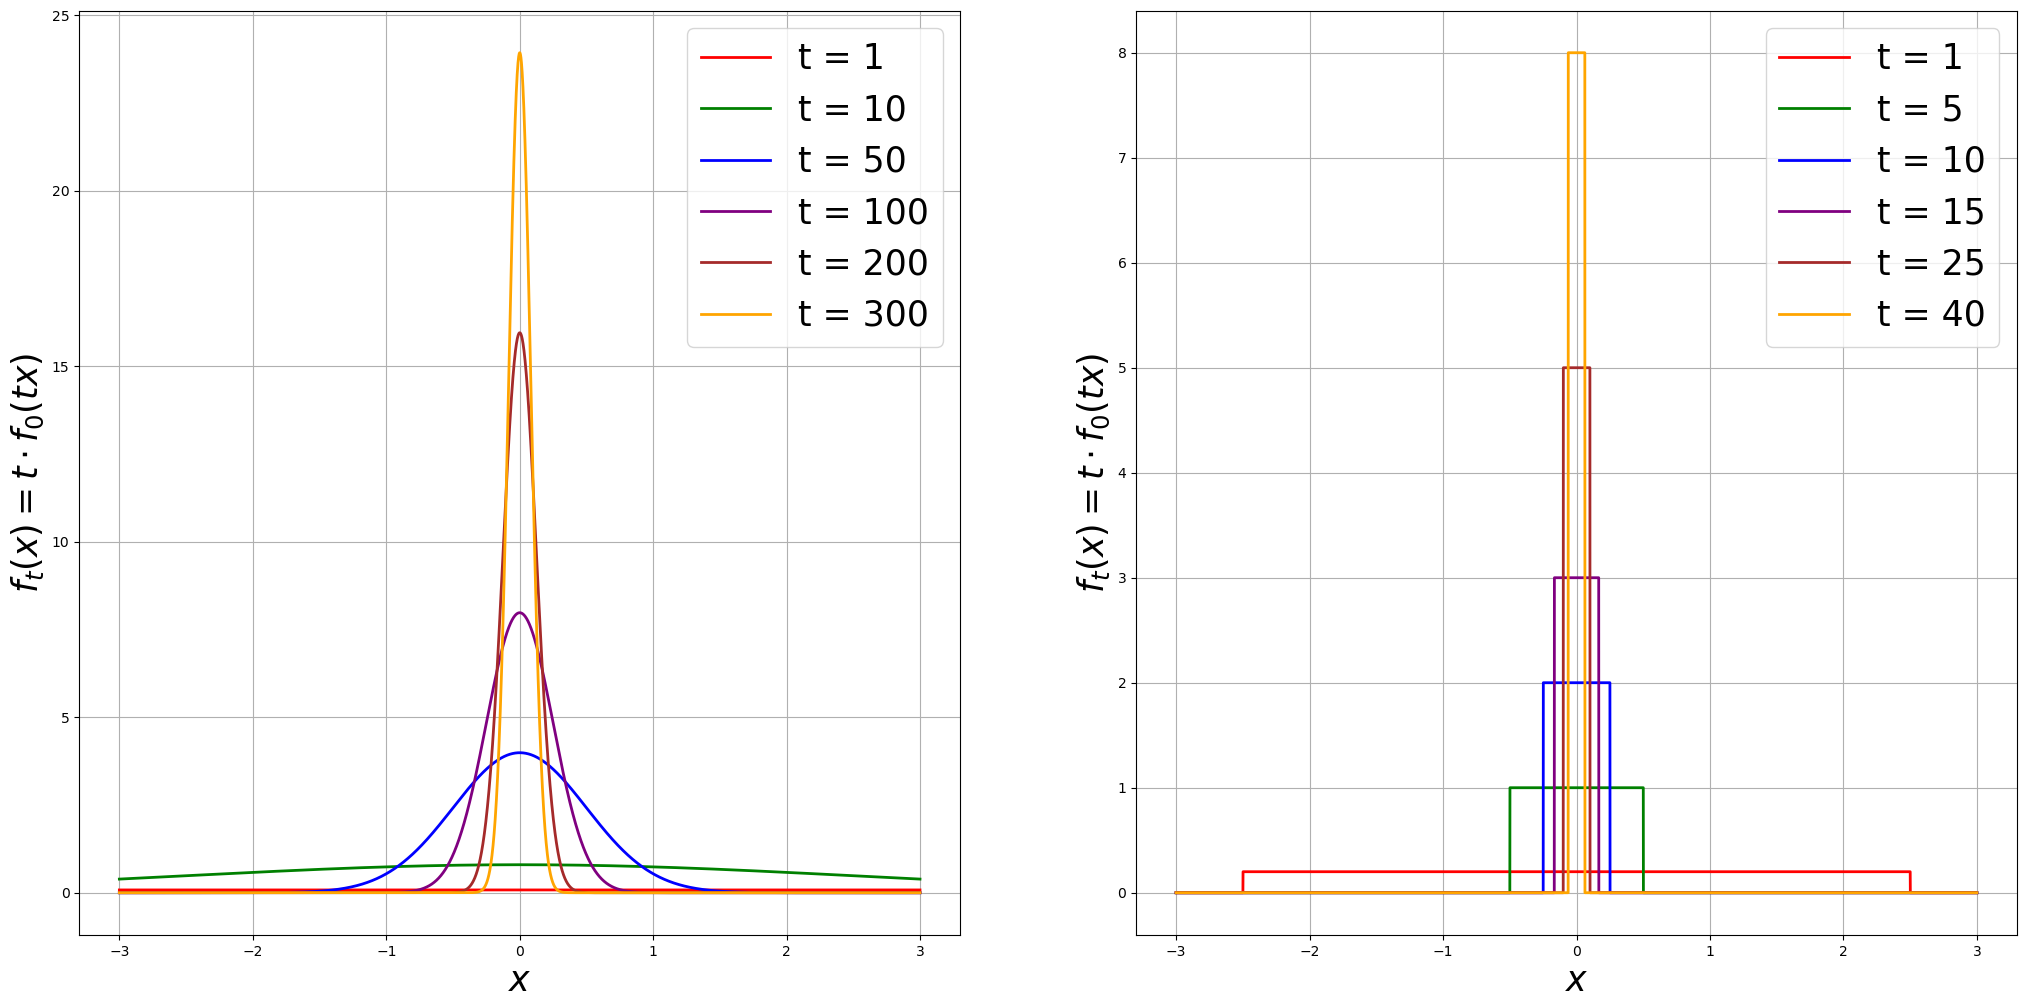
\includegraphics[width = 0.99\linewidth]{pictures/example1.png}
        \caption{Illustration of weak limit to $\delta$ function. $\mathcal{N}(0, 5)$ left, $\mathcal{U}[-2.5, 2.5]$ right.}
        \label{example1}
    \end{figure}

    

    


    

\section{Experiments} \label{Experiments}

    \subsection{Experiment Design} \label{design}
        We consider such a formulation of the problem of repeated supervised learning: there is an original data $\textbf{X}$ and a vector of target variables $\mathbf{y}$. Initially, at round $r = 0$, we select $30\%$ of the original dataset on which our model $f(\mathbf{x}, \theta^0)$ is trained with $80\%$ train size. 
        
        Then at each step $t$ we randomly select an element $(\mathbf{x^i}, y_i)$ -- the features and target variable of the $i$-th object from the original dataset, and this element does not lie in the initial dataset. Next, we get the prediction $y'_i$ of our model on the element $(\mathbf{x^i}, y_i)$: $y_i'=f(\mathbf{x^i}, \mathbf{\theta}^r)$ and sample $z_i \sim \mathcal{N}(y_i', s \cdot \sigma^2)$, where $s$ is an experiment parameter that indicates adherence. Then we remove 1 element from the active dataset and, with the probability of $p$, we add $(\mathbf{x^i}, z_i)$ to it, and with the probability $(1-p)$ we add the element $(\mathbf{x^i}, y_i)$. We carry out this procedure until we run out of elements that were not initially included in our dataset, so, we make a total of $0.7 \cdot n$ steps, where $n$ is the number of objects in $\textbf{X}$.

        After each $T$ steps round $r$ is increasing: $r = r+1$ and the machine learning model $f(x, \theta)$ is retrained with $80\%$ train size on active dataset. 

        The size of active dataset will always be $0.3 \cdot n$, because on each step we remove 1 element and add 1 element to active data. This experiment design is similar to \cite{khritankov2021hidden} were author was detecting hidden feedback loops in machine learning systems.

        In this paper we consider linear model, that is solved as Ridge with mean squared error loss function. In the formulation of our experiment, we consider $\mathbf{R}$ \eqref{R} as space of density functions of random vectors $(\mathbf{x^i}, y_i)$, where $\mathbf{x^i} \in \textbf{X}$ and $y_i \in \textbf{y}$ -- the features and target variable of the $i$-th object. The operator $\text{D}$ transforms $\mathbf{R}$ at each step $t$, and the distribution of features does not change, because at each step we take new $\mathbf{x^i}_t$ from the original set of features $\textbf{X}$, so only the distribution of the target variable changes. So we can use results from Theorem \ref{delta}. 

        In almost all distributions, decreasing the variance to 0 means that the distribution function takes the form of a delta function, for example in the normal distribution $\mathcal{N}(\mu, \sigma^2)$:

        \begin{equation*}
            f(x) = \dfrac{1}{\sqrt{2 \pi} \sigma} \exp\left[-\dfrac{1}{2} \cdot \left(\dfrac{x - \mu}{\sigma}\right)^2\right] \quad \text{ and } \quad \sigma^2 = \sigma^2
        \end{equation*}

        And in continuous uniform distribution $\mathcal{U}[a, b]$:
        \begin{equation*}
            f(x) = \dfrac{1}{b-a} \cdot \textbf{1}_{[a;b]} \quad \text{ and } \quad \sigma^2 = \dfrac{1}{12} \cdot (b-a)^2
        \end{equation*}

        For this reason, in our experiments every $N$ steps we measured the standard deviation in the $\mathbf{y} - \mathbf{y_{\text{pred}}}$ array, where $\mathbf{y_{\text{pred}}}$ is the predictions of our model on the active dataset. We measured the standard deviation at different \textit{usage} -- the probability with which we take $(\mathbf{x^i}, z_i)$ into the active dataset, and \textit{adherence} -- the parameter by which we multiply $\sigma^2$ when sampling $z_i$.

    \subsection{Experiment results} \label{res}
        First we consider $\mathbf{X}$ and $\mathbf{y}$ as a regression problem, so $\mathbf{y} = \mathbf{X}  \cdot \mathbf{\theta}$ for some vector $\mathbf{\theta}$. To complicate the model, a normally distributed noise was added to the data. This 3-dimensional plot will illustrate our results
        

\bibliographystyle{plain}
\bibliography{refs}  

\end{document}